%% generato automaticamente da tools/build_tex.py --- non modificare
\chapter{Quanto vale un gradino nel punto in cui salta}
\label{cap:u0-sign0}
\quaderno{u(0)-sign(0).dfw}{04 Jan 2011}{12}

Gennaio 2011. Il nome del file pone la domanda: quanto valgono, nell'origine, il gradino unitario $u$ e la funzione segno? La risposta convenzionale è $u(0)=1/2$ e $\mathrm{sgn}(0)=0$, scelta per simmetria. Il quaderno però arriva da un'altra strada — quella delle costruzioni di \dfw{mate.dfw} (capitolo~\ref{cap:mate}), dove il gradino nasceva come rapporto $\ln\!\left(\ldots\right)/x$ che nell'origine è una forma indeterminata — e le dodici righe che seguono confrontano quattro candidati.

Il quaderno non registra da quale funzione ciascun candidato provenga: si limita ai numeri e alle loro differenze. Le forme chiuse qui sotto sono ricostruite dai valori.

\section{I quattro candidati}

Le prime otto righe calcolano i quattro valori. Espressi in forma chiusa sono $\ln(\mathrm{e}-1)$, $\ln\sinh 1$, la media fra quest'ultimo e $1$, e il doppio del primo diminuito di uno.

\begin{espr}{1}{User}{}
\[
\ln\!\left(\mathrm{e} - 1\right)
\]
\end{espr}
Il primo candidato: $\ln(\mathrm{e}-1)$.

\begin{espr}{2}{Approx(\#1)}{}
\[
0.5413248546
\]
\end{espr}
Vale $0{,}5413248546$: poco più di un mezzo.

\begin{espr}{3}{User}{}
\[
\ln\!\left(\frac{\mathrm{e}^{2} - 1}{2\, \mathrm{e}}\right)
\]
\end{espr}
Il secondo candidato. L'argomento del logaritmo è $\sinh 1$.

\begin{espr}{4}{User}{}
\[
0.1614393615
\]
\end{espr}
Vale $0{,}1614393615$.

\begin{espr}{5}{User}{}
\[
0.5\, \left(\ln\!\left(\frac{\mathrm{e}^{2} - 1}{2\, \mathrm{e}}\right) + 1\right)
\]
\end{espr}
La media fra il secondo candidato e l'unità.

\begin{espr}{6}{Approx(\#5)}{}
\[
0.5807196807
\]
\end{espr}
Vale $0{,}5807196807$.

\begin{espr}{7}{User}{}
\[
2\, \ln\!\left(\mathrm{e} - 1\right) - 1
\]
\end{espr}
Il doppio del primo candidato, meno uno: è la trasformazione che porta dal gradino al segno.

\begin{espr}{8}{Approx(\#7)}{}
\[
0.08264970922
\]
\end{espr}
Vale $0{,}0826497092$.

\begin{figure}[htbp]
  \centering
  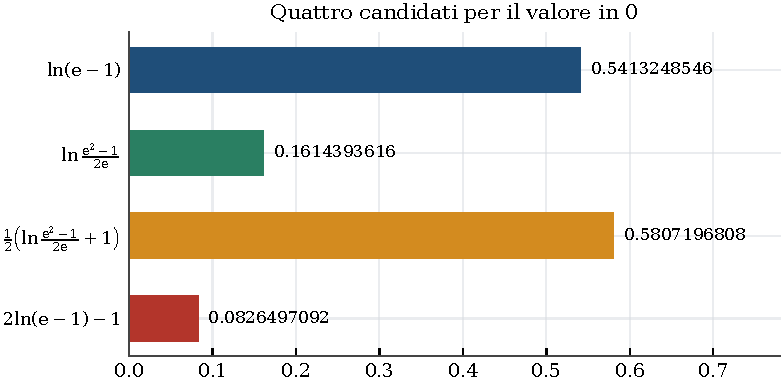
\includegraphics[width=0.86\linewidth]{../figures/u0.pdf}
  \caption{I quattro candidati a confronto. La convenzione usuale porrebbe il gradino a $0{,}5$; il candidato più vicino, $\ln(\mathrm{e}-1)$, la supera di quattro centesimi.}
  \label{fig:u0}
\end{figure}

I quattro numeri sono $0{,}5413$, $0{,}1614$, $0{,}5807$ e $0{,}0826$. Il secondo si riconosce subito: $\dfrac{\mathrm{e}^2-1}{2\mathrm{e}}=\dfrac{\mathrm{e}-\mathrm{e}^{-1}}{2}=\sinh 1$, dunque la riga $\#3$ è $\ln\sinh 1$. Il primo è $\ln(\mathrm{e}-1)$ e vale poco più di un mezzo, il che lo rende il candidato più vicino alla convenzione usuale per $u(0)$.

Le righe $\#5$ e $\#7$ sono due modi diversi di normalizzare: la prima fa la media fra $\ln\sinh1$ e $1$, la seconda raddoppia $\ln(\mathrm{e}-1)$ e sottrae $1$. Sono le stesse due operazioni che in \dfw{mate.dfw} portavano dal gradino alla funzione segno e viceversa.

\section{Le due differenze}

Le ultime quattro righe confrontano i candidati a coppie, e qui c'è una relazione esatta.

\begin{espr}{9}{User}{}
\[
0.5\, \left(\ln\!\left(\frac{\mathrm{e}^{2} - 1}{2\, \mathrm{e}}\right) + 1\right) - \ln\!\left(\mathrm{e} - 1\right)
\]
\end{espr}
La differenza fra il terzo e il primo candidato.

\begin{espr}{10}{Approx(\#9)}{}
\[
0.03939482617
\]
\end{espr}
Vale $0{,}0393948262$, cioè $\tfrac12\ln\!\left[\coth(1/2)/2\right]$.

\begin{espr}{11}{User}{}
\[
\ln\!\left(\frac{\mathrm{e}^{2} - 1}{2\, \mathrm{e}}\right) - \left(2\, \ln\!\left(\mathrm{e} - 1\right) - 1\right)
\]
\end{espr}
La differenza fra il secondo e il quarto.

\begin{espr}{12}{Approx(\#11)}{}
\[
0.07878965234
\]
\end{espr}
Vale $0{,}0787896523$, esattamente il doppio della riga $\#10$: i due scarti sono la stessa quantità misurata sulla scala del gradino e su quella del segno.


I due scarti stanno in rapporto esattamente $1$ a $2$: la riga $\#12$ vale il doppio della riga $\#10$, cifra per cifra. Non è una coincidenza numerica ma un'identità, e si vede sviluppando. Poiché $\sinh1=\dfrac{(\mathrm{e}-1)(\mathrm{e}+1)}{2\mathrm{e}}$, si ha $\ln\sinh1=\ln(\mathrm{e}-1)+\ln(\mathrm{e}+1)-\ln2-1$, e sostituendo:
\[
  \frac{\ln\sinh 1+1}{2}-\ln(\mathrm{e}-1)
  =\frac{1}{2}\ln\frac{\mathrm{e}+1}{2(\mathrm{e}-1)}
  =\frac{1}{2}\ln\frac{\coth\tfrac12}{2},
\]
mentre la riga $\#12$ dà lo stesso logaritmo senza il fattore un mezzo. Il valore comune è $\ln\coth\tfrac12-\ln2=0{,}0787896523\ldots$

Questo dice che i quattro candidati non sono indipendenti: due sono la stessa cosa a meno del riscalamento gradino-segno, e la loro distanza è la stessa quantità misurata su due scale diverse. Nessuno dei quattro vale $1/2$, e il più vicino, $\ln(\mathrm{e}-1)=0{,}5413$, se ne discosta di quattro centesimi.

\section*{In sintesi}
\addcontentsline{toc}{section}{In sintesi}

Il quaderno non conclude, e forse non poteva. La domanda «quanto vale un gradino nel punto in cui salta» non ha una risposta unica: dipende da quale famiglia di funzioni continue lo si consideri limite. La convenzione $1/2$ nasce dalla simmetria e dalla serie di Fourier; i valori raccolti qui nascono invece dalle costruzioni logaritmiche di \dfw{mate.dfw}, e sono diversi perché diverso è il limite. L'unica cosa che le dodici righe stabiliscono con certezza è la relazione esatta fra i due scarti — e quella, almeno, è un'identità.

